% E: x^2/4+y^2=1; Gamma: (x-1)^2+y^2=4.
% Intersections x=(4-2sqrt(10))/3; y=+-sqrt(1-x^2/4).
\begin{center}
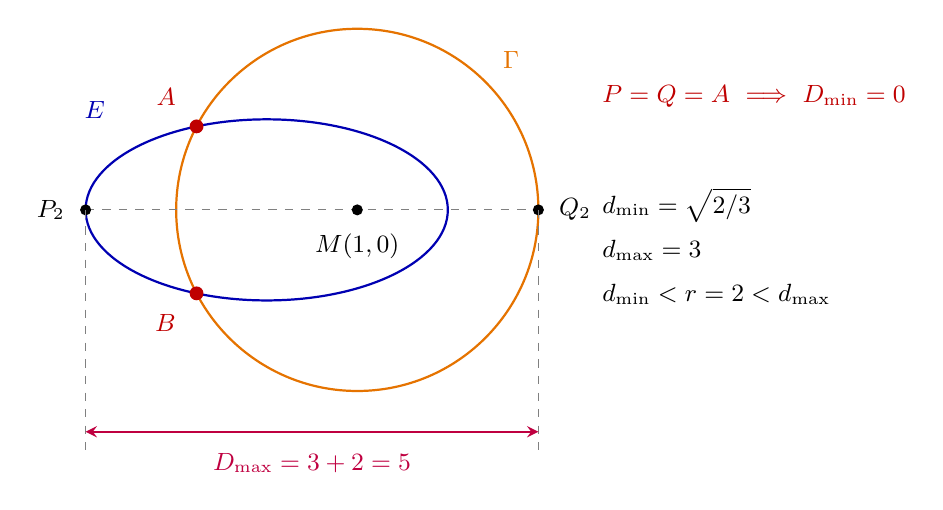
\begin{tikzpicture}[x=1.15cm,y=1.15cm,>=stealth,font=\small]
\pgfmathsetmacro{\ix}{(4-2*sqrt(10))/3}
\pgfmathsetmacro{\iy}{sqrt(1-\ix*\ix/4)}
\draw[blue!70!black,thick] (0,0) ellipse (2 and 1);
\draw[orange!90!black,thick] (1,0) circle (2);
\draw[gray,dashed] (-2,0)--(3,0);
\fill (1,0) circle(2pt) node[below=5pt] {$M(1,0)$};
\fill (-2,0) circle(2pt) node[left=4pt] {$P_2$};
\fill (3,0) circle(2pt) node[right=4pt] {$Q_2$};
\fill[red!75!black] (\ix,\iy) circle(2.5pt) node[above left=4pt] {$A$};
\fill[red!75!black] (\ix,-\iy) circle(2.5pt) node[below left=4pt] {$B$};
\node[red!75!black,anchor=west] at (3.6,1.25) {$P=Q=A\ \Longrightarrow\ D_{\min}=0$};
\node[blue!70!black] at (-1.9,1.1) {$E$};
\node[orange!90!black] at (2.7,1.65) {$\Gamma$};
\draw[gray,dashed] (-2,0)--(-2,-2.65) (3,0)--(3,-2.65);
\draw[<->,purple,thick] (-2,-2.45)--(3,-2.45)
 node[midway,below=4pt] {$D_{\max}=3+2=5$};
\node[anchor=west,align=left] at (3.6,-.4)
 {$d_{\min}=\sqrt{2/3}$\\[5pt]$d_{\max}=3$\\[5pt]$d_{\min}<r=2<d_{\max}$};
\end{tikzpicture}
\end{center}
